% !TeX root = ../../main.tex
\section{Kinetics}
\subsection{Nitration of toluene}
The nitrotoluene production was achieved by  reacting 95\% w/v toluene and 70 \% w/v nitric acid to produce 3 different nitrotoluene isomers of ONT, MNT and PNT in a heat-exchanger tubular reactor operating at 330K and X atm. 
\begin{scheme}[h]
    \centering
    \ch{ TOL + HNO3 -> ONT + MNT + PNT + H2O}
    \caption{Toluene nitration to nitrotoluene isomers}
    \label{eqn: nitration}
\end{scheme}

The nitration of toluene is governed by intrinsic kinetics under the experimental conditions [Jeeru et al]. The rate equation can be defined as  

\begin{equation}
-\frac{d C_{Toluene}}{d t} = k_{2} C_{Toluene} C_{Nitric Acid} \approx k_{1} C_{Toluene}
\end{equation}

where $k_2$, $k_1$ are the second-order and pseudo-first order rate constant respectively. A pseduo-first order rate constant can be assumed since nitric acid is in excess. The electrophilic substitution between the nitronium ion and toluene is the rate determining step [carey and sundberg].

\begin{figure}[h]
    \centering
    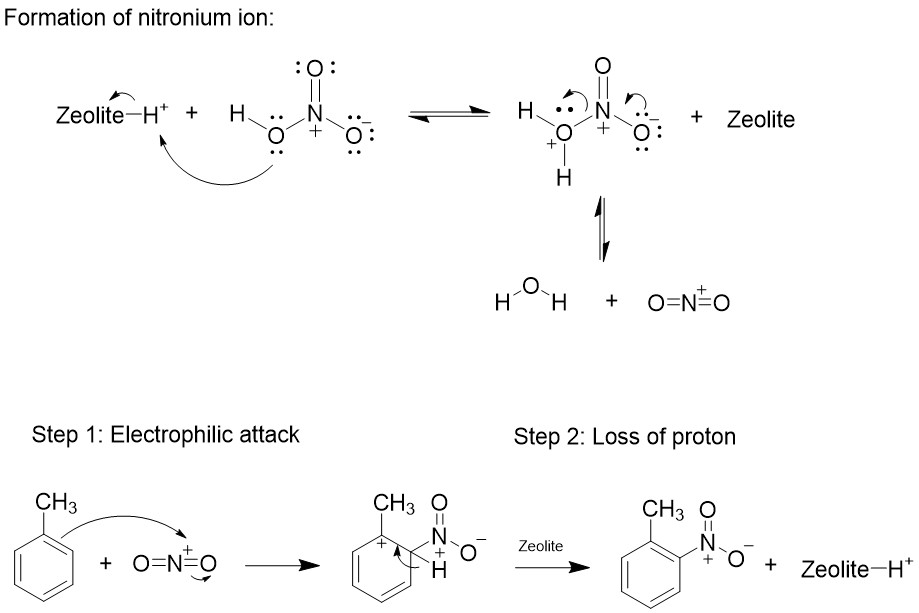
\includegraphics[width=\linewidth]{chapters/2-reaction/figures/Nitration.jpg}
    \caption{Mechanism for nitration of toluene to \ortho-nitrotoluene. Mechanism for meta- and \para-nitrotoluene are similar, expect that the nitronium ion attacks the \meta and \para position of the toluene respectively}
    \label{fig:finalroutes}
\end{figure}

Nitric acid interacts with the Brønsted acid sites on H-Mordenite by forming a hydrogen bond with the \ch{H+} proton [chary et al]. This results in a intermediate nitronium ion \ch{NO2+} and water molecule \ch{H2O}. The nitronium ion then undergoes electrophilic substitution with the aromatic ring of toluene to form nitrotoluenes. The electron-donating inductive effect of the methyl group on toluene favors \ortho and \para positions for nitrotoluene.

\subsection{Hydrogenation of o-nitrotoluene}
After the production of the 3 nitrotoluene isomers, (mention separation?) ONT is mixed with propanol and hydrogenated to o-TOL in a co-current trickle bed reactor operating at 333K and 3 atm. 

\begin{scheme}[h]
    \centering
    \ch{ ONT + 3 H2 -> O{-}TOL + 2 H2O }
    \caption{ONT hydrogenation to O-TOL}
    \label{eqn: ONT hydrogenation}
\end{scheme}

include ChemDraw here
The rate equation for this equation can be defined as: 
\begin{equation}
    r = k P_{H_2}^{0.3} 
    \label{ONT rate equation}
\end{equation}
 \begin{equation}
     k = 211.69 exp(-\frac{45.52 \cdot 10^{3}}{RT} \frac{mol}{kPa^{0.3}g_{cat}s})
 \end{equation}
\subsection{Oxidation of p-nitrotoluene}
\subsection{Hydrogenation of nitrobenzaldehyde and nitrobenzoic acid}